% Brief report style paper

% It's about how a somatotopically ordered pattern can be
% re-established in the cortex based on information carried with
% thalamocortical axons afferent from the ventrobasal thalamus, but
% without specifying absolute positions as centre-points for the
% barrels. Everything in the paper should be tailored towards arguing
% this idea.

\documentclass[9pt,twocolumn,twoside,lineno]{pnas-new}
\templatetype{pnasresearcharticle}

\title{Modelling the emergence of whisker barrels}
% While writing, don't stop for errors
%\nonstopmode


% Use letters for affiliations, numbers to show equal authorship (if applicable) and to indicate the corresponding author
\author[a,1]{Sebastian~S.~James}
\author[b]{Leah A. Krubitzer}
\author[a]{Stuart~P.~Wilson}

\affil[a]{Department of Psychology, The University of Sheffield, Sheffield, United Kingdom.}
\affil[b]{Center for Neuroscience, The University of California, Davis, United States.}
% $^{*}$Corresponding author email: Seb.James@Sheffield.ac.uk\vspace{1em}\\

\leadauthor{James}

\correspondingauthor{\textsuperscript{1}To whom correspondence should be addressed. E-mail: \href{mailto:seb.james@sheffield.ac.uk}{\nolinkurl{seb.james@sheffield.ac.uk}}}

\keywords{Barrel cortex $|$ Self-organization $|$ Somatotopic map $|$ Axon guidance}

\begin{abstract}
Brain development relies on an interplay of genetic specification and self-organisation. Striking examples of this interplay can be found in the rodent somatosensory brainstem, thalamus, and cortex, where the arrangement of the facial whiskers is preserved in the arrangement of cell aggregates to form precise somatotopic maps. We show in simulation how realistic whisker maps can self-organize, by assuming that information is exchanged between adjacent cells only, under the guidance of gene expression gradients. The resulting model provides a simple account of how genetic information can constrain spontaneous pattern formation to faithfully reproduce functional maps in subsequent brain structures.
\end{abstract}

\dates{This manuscript was compiled on \today}
\doi{\url{www.pnas.org/cgi/doi/10.1073/pnas.XXXXXXXXXX}}

\begin{document}

% Blue for comments
\newcommand{\cmnt}[1]{\textcolor{blue}{#1}}
\newcommand{\dvrg}{\nabla\vcdot\nabla}
\newcommand{\e}{\emph}
\newcommand{\bol}{\textbf}
\newcommand{\mb}[1]{\mathbf{#1}}
\makeatletter
\newcommand*\vcdot{\mathpalette\vcdot@{.35}}
\newcommand*\vcdot@[2]{\mathbin{\vcenter{\hbox{\scalebox{#2}{$\m@th#1\bullet$}}}}}
\makeatother

\maketitle
\thispagestyle{firststyle}
\ifthenelse{\boolean{shortarticle}}{\ifthenelse{\boolean{singlecolumn}}{\abscontentformatted}{\abscontent}}{}

\modulolinenumbers{}
\linenumbers

\dropcap{S}patial patterns in neural connectivity provide clues about the constraints under which brains evolve and develop \citep{purves_iterated_1992}. Perhaps the most distinctive pattern can be found in the rodent barrel cortex \cite{woolsey_structural_1970}. The barrels are large cortical columns, identifiable from birth in layer 4 of primary somatosensory cortex as dense clusters of thalamocortical axons, which are enclosed by borders a few neurons thick from postnatal day 3 \citep{erzurumlu_development_2012}. In the plane tangential to the cortical surface the barrels constitute a somatotopic map of the whiskers, with cells of adjacent barrels responding most strongly and quickly to deflection of adjacent whiskers \citep{armstrong-james_flow_1992}. Barrel patterning reflects subcortical whisker maps comprising cell aggregates called barrelettes in the brainstem and barreloids in the thalamus.
%\cite{van_der_loos_barreloids_1976}.

Barrel formation requires afferent input from whisker stimulation and thalamic calcium waves \citep{anton-bolanos_prenatal_2019}, and depends on a complex network of axon guidance molecules such as ephrin-A5 and A7 and adhesion molecules such as cadherin-6 and 8 \citep{vanderhaeghen_mapping_2000,miller_epha7-ephrin-a5_2006}.
This network is orchestrated by interactions between morphogens Fgf8 and Fgf17 and transcription factors Emx2, Pax6, Sp8, and Coup-tf1 \citep{shimogori_fibroblast_2005}, which are expressed in gradients that mark orthogonal axes and can be manipulated to stretch, shrink, shift, and even duplicate barrels \cite{assimacopoulos_fibroblast_2012}.
% Removed ref: ,bishop_regulation_2000 after ..Coup-tf1

The barrel boundaries form a Voronoi tessellation across the cortical sheet \citep{senft_mouse_1991} (Fig.\,1A), suggesting that barreloid topology is preserved in the projection of thalamocortical axons into the cortex, and that a barrel forms by lateral axon branching from an initial centre-point that ceases upon contact with axons branching from adjacent centres. But the assumption of pre-arranged centres is difficult to resolve with the observation that  axons arrive in the cortical plate as an undifferentiated bundle, prior to barreloid formation \cite{agmon_organized_1993}.

Alternatively, reaction-diffusion dynamics could generate a Voronoi tessellation without pre-arranged centres, by amplifying characteristic modes in a noisy initial distribution of axon branches, as a net effect of short-range cooperative and longer-range competitive interactions. Accordingly, the barrel pattern would be determined by the relative strength of these interactions and by the shape of the cortical field boundary. However, intrinsic cortical dynamics alone cannot account for the topographic correspondence between thalamic and cortical domains, the irregular sizes and specific arrangement of the barrels in rows and arcs, or the influence of gene expression gradients.

The centre-point and reaction-diffusion models are not mutually exclusive. Pre-organised centres could bias reaction-diffusion processes to generate specific  arrangements more reliably, and mechanisms of lateral axon branching may constitute the tension between cooperation and competition required for self-organization. However, proof that barrel patterning can emerge from an undifferentiated bundle of  axons, based only on local interactions, would show that a separate stage and/or extrinsic mechanism for pre-organising thalamocortical connections need not be assumed. To this end, we ask whether barrel maps can emerge in a system with reaction-diffusion dynamics, under the guidance of signalling gradients, and in the absence of pre-defined centres.


\section*{Models}

Karbowski \& Ermentrout \citep{karbowski_model_2004} developed a reaction-diffusion style model of how extrinsic signalling gradients can constrain the emergence of distinct fields from intrinsic cortical dynamics. Their model defines how the density of connections $c(x,t)$ and axon branches $a(x,t)$ interact at time $t$, along a 1D anterior-posterior axis $x$, for $N$ thalamocortical projections indexed by $i$. The model was derived from the assumption that the rates at which $a_i$ and $c_i$ grow are reciprocally coupled. Extending the original 1D model to simulate arealization on a 2D cortical sheet, we use $a_i(\mb{x},t)$ and $c_i(\mb{x},t)$, and model synaptogenesis as
%
\begin{equation} \label{eq:dc}
\frac{\partial c_i}{\partial t} =-\alpha c_i +\beta  \left(1 - \sum_{j=1}^{N} c_{j}\right)[a_i]^k.
\end{equation}
%
Accordingly, where the total density of synaptic connections sums to one, connections decay at rate $\alpha$. Otherwise the connection density increases non-linearly ($k>1$) with the density of axon branching. Axon branching is modelled as
%
\begin{equation} \label{eq:da}
\frac{\partial a_i}{\partial t} = \nabla\vcdot\left(D \nabla a_i-a_i\sum_{j=1}^{M} \gamma_{i,j}\nabla \rho_j(\mb{x})\right) - \frac{\partial c_i}{\partial t} + \chi_i.
\end{equation}
%
The first term on the right describes the divergence (indicated by $\nabla\vcdot$) of the quantity in parentheses, which is referred to as the `flux' of axonal branching. The flux represents diffusion across the cortical sheet, at rate $D$, and the influence of $M$ molecular signalling fields, $\rho(\mb{x})$. The influence of a given field (indexed by $j$) on a given thalamic projection (indexed by $i$), is determined by $\gamma_{i,j}$, which may be positive or negative in order that axons may branch in the direction of either higher or lower  concentrations. The second term on the right represents an assumption that axon branching decreases when synaptogenesis increases, and vice versa, i.e., that axon branches are required for synaptic connections to form. Here $\chi_i=0$ is a placeholder.

Software for modelling the cortical sheet as a hexagonal lattice with no-flux
boundary conditions and an arbitrary boundary shape, for computing the flux
using a finite difference method, for numerical integration by the
fourth-order Runge-Kutta method, and for reproducing these results is available at \url{https://github.com/ABRG-Models/BarrelEmerge}.

\section*{Results}

\begin{figure*}
\begin{center}
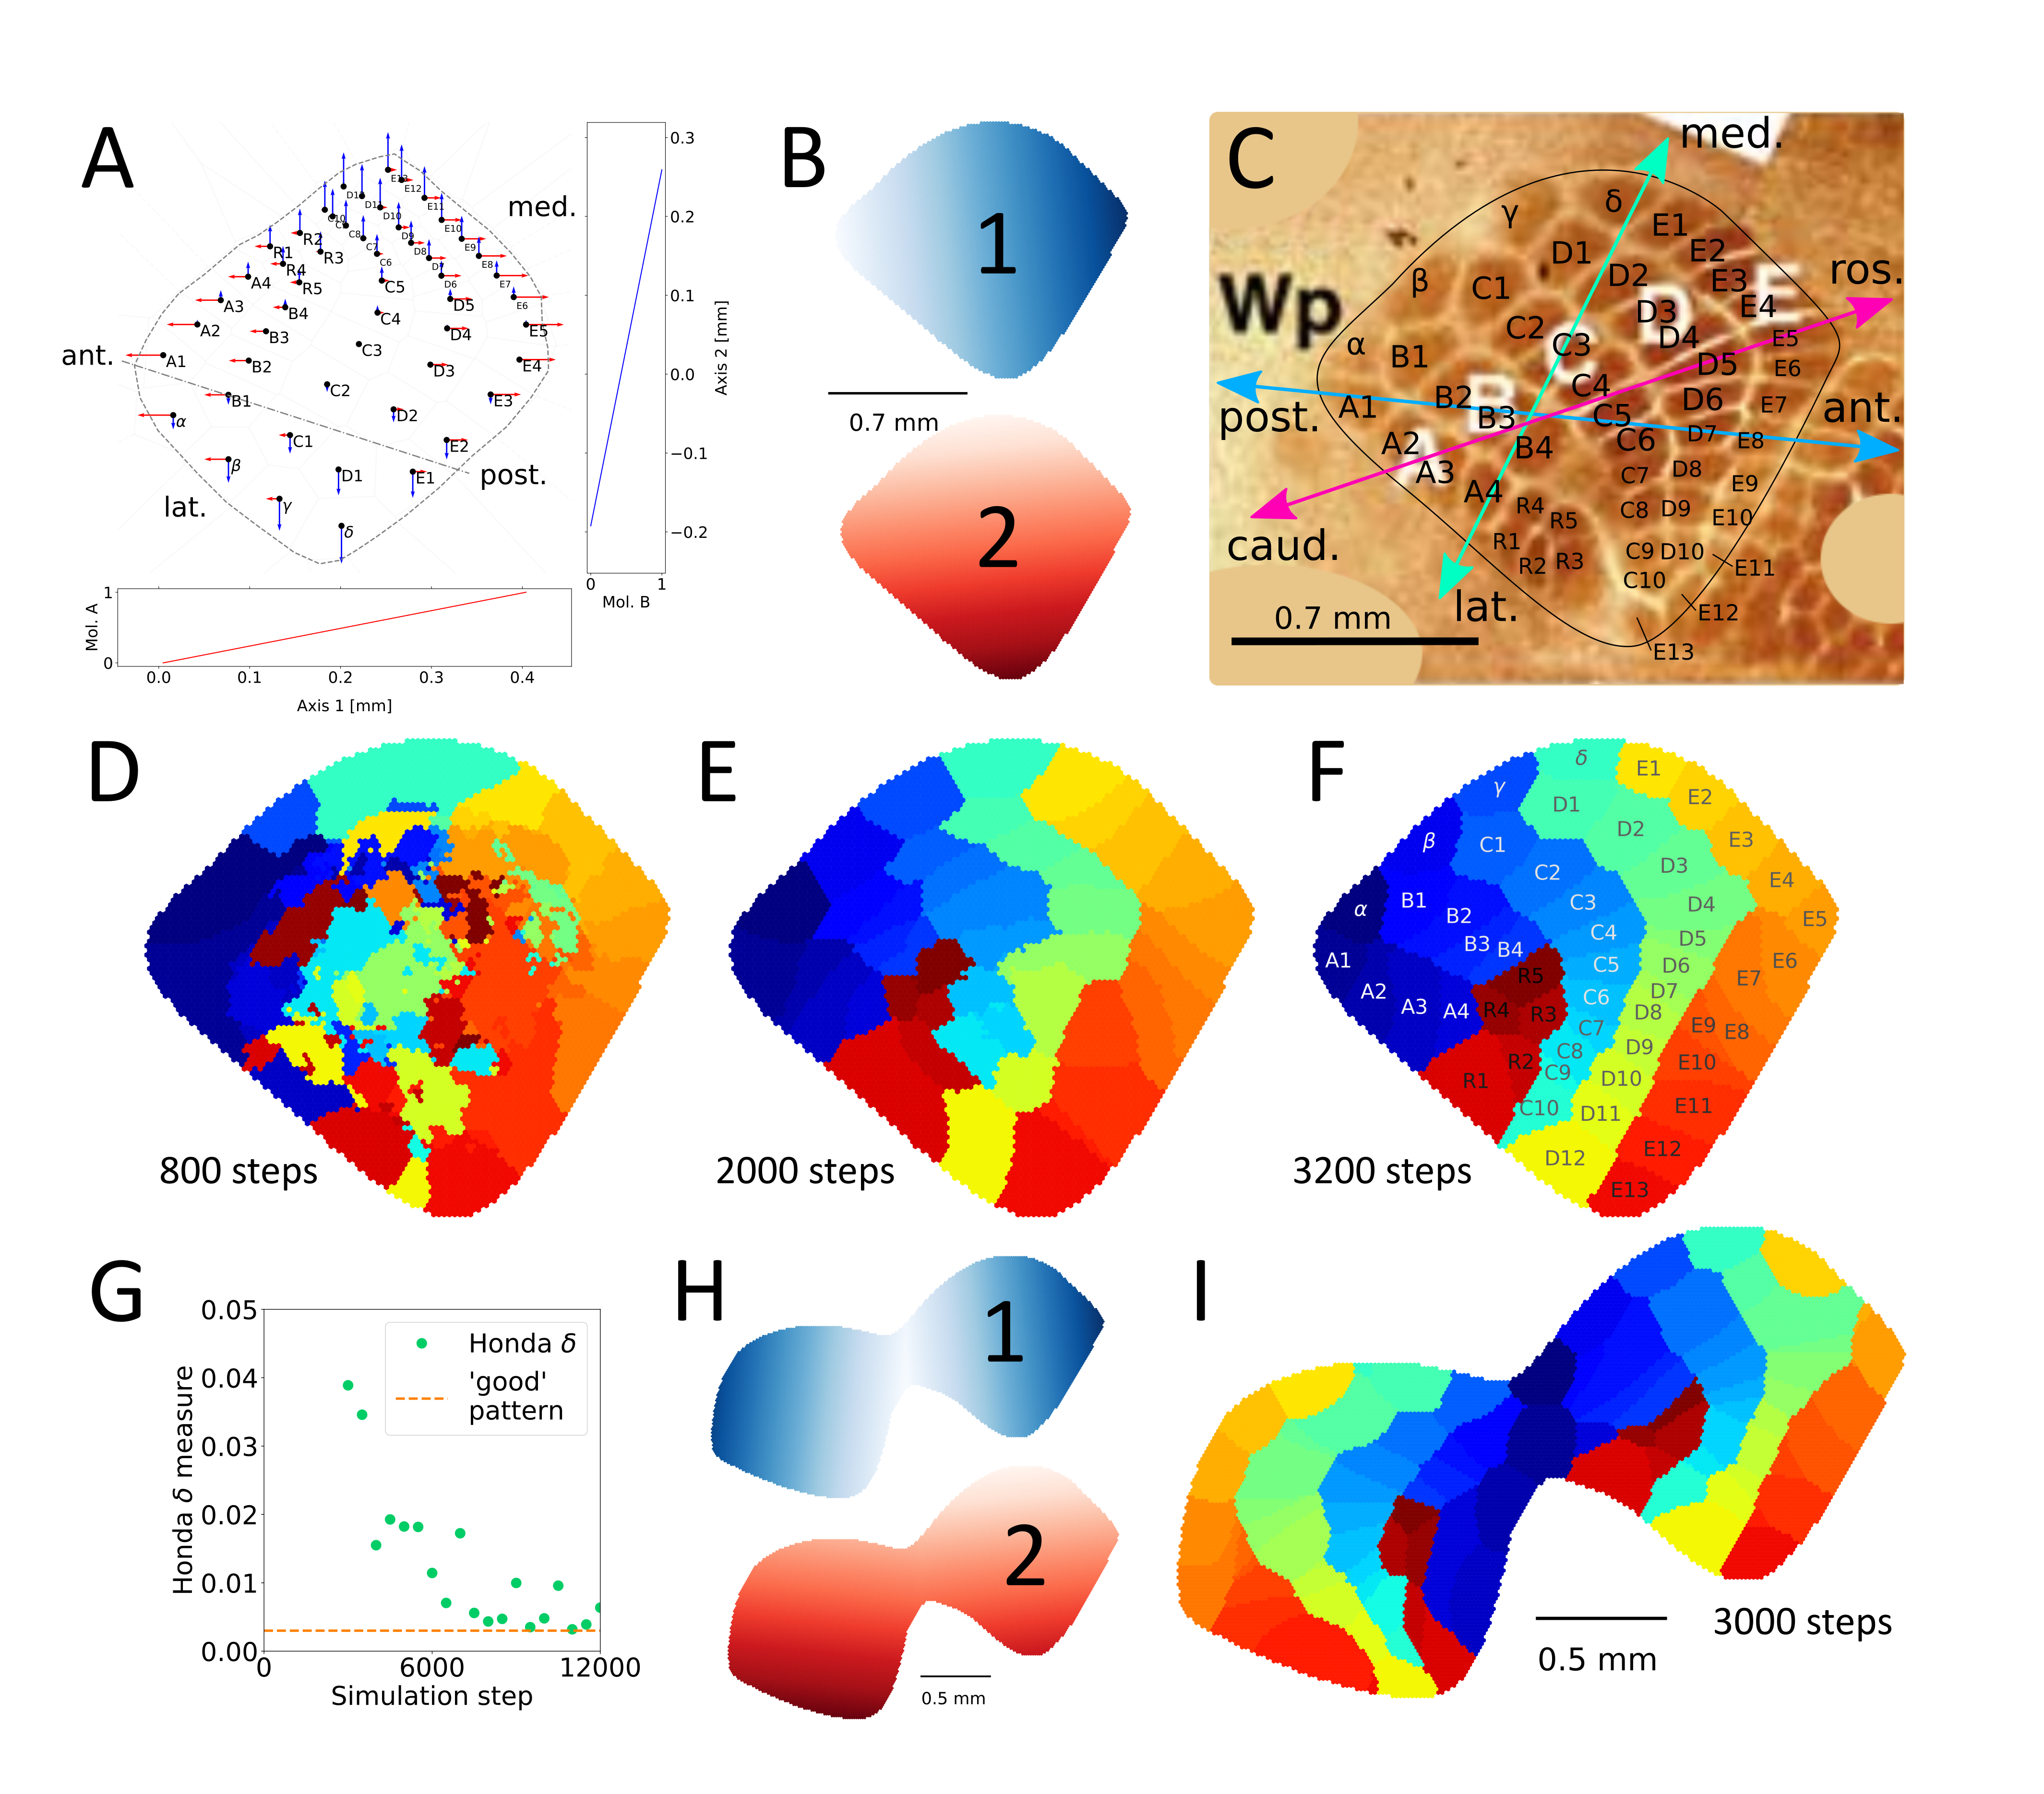
\includegraphics[width=0.8\textwidth]{./MainFig.png}
\end{center}
\caption{\textbf{A} Left shows a cytochrome oxidase stain obtained from rat S1 by \cite{zheng_signal_2001}, with black lines to delineate barrels and to measure departure ($\delta$) from a perfect Voronoi tesselation. Right shows the initial distribution of axon branching density ($a$) for one thalamocortical projection and two molecular guidance fields ($\rho$). \textbf{B} The strength of interaction $\gamma$ for each of 41 projections with field $\rho_1$ and $\rho_2$ are indicated by the lengths of green and blue arrows respectively, assuming that similar fields aligned to the posterior-anterior and medial-lateral axes in the ventroposterior medial nucleus of the thalamus are sampled at the locations of barreloid centers (reconstructed from \cite{haidarliu_size_2001}). \textbf{C} Simulation results for parameters $N=41$, $\alpha=3$, $\beta=20$, $k=3$, $D=0.2$, $\gamma\in\pm 2$ and $\delta{t}=0.0001$. Colours indicate the thalamic projection for which the connection density is maximal, black lines delineate boundaries, and overlaid contours show $c>0.5$. \textbf{D} The Honda $\delta$ metric (red dots; see \cite{senft_mouse_1991}) measures departure from a Voronoi tesselation (dotted line corresponds to the barrels in $A$), and $\eta$ (black squares) measures the correspondence between the real and simulated barrel shapes (the product of the sum of squared differences between real and simulated centers and the sum of differences in area; units mm$^4$). \textbf{E.} Guidance fields and emergent barrel pattern in a Fgf8 misexpression experiment (c.f. \cite{assimacopoulos_fibroblast_2012}), simulated by reflecting $\rho_1$ about the anterior-posterior axis. All scale bars 1mm.}
\label{fig:main}
\end{figure*}

First we verified that all results established by \cite{karbowski_model_2004} for a 1D axis could be reproduced using our extension to a 2D cortical sheet. Using an elliptical boundary with $M=3$ offset guidance gradients aligned to the longer axis, $N=5$ thalamocortical projections gave rise to five distinct cortical fields at locations that preserved the topographic ordering defined by the original $\gamma$ values. However, we found that specifying $N$ ordered areas required $M\approx (N+1)/2$ signalling fields. As the number of distinct guidance fields is unlikely to approach the number of barrels, further extensions were required.

The term in parentheses in Eq.~\ref{eq:dc} represents competition between thalamocortical projections for a limited availability of cortical connections. To introduce competition also in terms of axon branching we redefined
%
\begin{equation} \label{eq:comp}
\chi_i(\mb{x}, t) = - \frac{\epsilon  a_i}{N-1} \sum_{j \ne i}^{N} a_{j},
\end{equation}
%
which reduces branching for each projection where the branches of other projections are dense. Divisive normalization keeps the axon branch density bounded on each iteration to the initial density  at $t=0$;
%
\begin{equation} \label{eq:norm}
  a_i(\mathbf{x}, t) = \int_\Omega  a_i(\mathbf{x}, 0) d\sigma \; \frac {a'_i(\mathbf{x}, t)} {\int_\Omega
  a'_i(\mathbf{x}, t) d\sigma},
\end{equation}
%
where prime symbols indicate the use of intermediate values computed from Eqs.~\ref{eq:dc}--\ref{eq:comp} at time $t-{\delta}t$.

The only differences between thalamic projections are their strengths of interaction with the guidance fields, $\gamma$, hence any reliable differences between emergent cortical fields must be due to differences in these values only. We speculate that a projection interacts with a given ephrin field in the cortical subplate with a strength determined by the concentration of a similar molecule at its thalamic origin, i.e., the putative barreloid center. As such, two orthogonal linear thalamic gradients were defined, from which 41 pairs of $\gamma$ values were sampled, at the coordinates of 41 barreloid centers recreated from \cite{haidarliu_size_2001} (Fig.\,1B).

A cortical boundary enclosing 41 corresponding barrels was traced from a cytochrome oxidase stain from \cite{zheng_signal_2001}, and Eqs.~\ref{eq:dc}--\ref{eq:norm} were solved for $N=41$ projections on the resulting domain, using $M=2$ linear signalling gradients aligned with the anterior-posterior and medial-lateral axes. From random initial conditions for $a({\bf x},0)$ and $c({\bf x},0)$, a clear Voronoi-like tesselation emerged (Fig.\,1C). A reduction in the Honda delta metric (see \cite{senft_mouse_1991}) confirmed that a `good' Voronoi pattern emerged within $\approx 3000$ iterations (see Fig.\,1D). A measure of the difference in shape between real and simulated barrels revealed a strong correspondence (see Fig.\,1D).

To further investigate the interplay of genetic and intrinsic mechanisms we simulated a seminal barrel duplication experiment \cite{shimogori_fibroblast_2005},  first by solving on a cortical domain comprising two separate, identically shaped cortical boundaries. In this case one distinct cortical field per thalamic projection emerged, within one of the two boundaries only, i.e., no duplication. However, merging the two fields to create an extended mirror-symmetric boundary shape, with an anterior-posterior guidance field reflected at the join, gave rise to two mirror-symmetrical barrel fields comprising 2N barrels, i.e., two cortical fields for each thalamic projection (Fig.\,1E). Together these results suggest that by the misexpression of Fgf8, Shimogori \& Grove \citep{shimogori_fibroblast_2005} effectively created one large barrel field rather than two distinct cortical fields.

\section*{Discussion}

The present results suggest that the key requirements for the emergence of realistic barrel patterning are i) at each cortical location thalamocortical projections compete for a limited number of available synaptic connections (Eqs.~\ref{eq:dc}--\ref{eq:da}), ii) at each location the branching rate of a given projection is reduced by the density of other projections (Eq.~\ref{eq:comp}), and iii) the branch density of each projection is conserved (Eq.~\ref{eq:norm}).

It is important to emphasize that the formulation of the model is entirely local, insofar as simulation requires no information to be communicated from a given cortical grid cell to any but those immediately adjacent (via diffusion). Hence the simulations demonstrate how a self-organising system, constrained by genetically specified guidance cues, can faithfully reproduce an arrangement of cell aggregates in one neural structure as a topographic map in another.
%
The model also shows that the shape of the barrels may be primarily determined
by the competitive and cooperative interactions between cells relative to the
shape of the cortical field boundary. And that somatotopic map formation does
not require the pre-specification of centre-points by as yet undetermined
additional developmental mechanisms.

\bibliography{../BarrelEmerge}

\end{document}
